\vspace{0.5em}
\section{Approach}

% APPROACH: Tell us how your implementation works. Your description should be sufficiently detailed to provide the course staff a basic understanding of your approach. Again, it might be very useful to include a figure here illustrating components of the system and/or their mapping to parallel hardware.
% Describe the technologies used. What language/APIs? What machines did you target?
% Describe how you mapped the problem to your target parallel machine(s). IMPORTANT: How do the data structures and operations you described in part 2 map to machine concepts like cores and threads. (or warps, thread blocks, gangs, etc.)
% Did you change the original serial algorithm to enable better mapping to a parallel machine?
% If your project involved many iterations of optimization, please describe this process as well. What did you try that did not work? How did you arrive at your solution? The notes you’ve been writing throughout your project should be helpful here. Convince us you worked hard to arrive at a good solution.
% If you started with an existing piece of code, please mention it (and where it came from) here.

In this section, we describe the implementation and parallelization of the tetris game solvers. First, we implemented sequential versions of depth-first search and breadth-first search solvers from scratch in C to be incorporated into the tetris game code \ref{ref:tetrisRepo}. Then, we parallelized both methods with OpenMP on the GHC machines and later conducted our experiments on the PSC bridges2 machines. We also built CilkPlus (\ref{ref:CilkPlus}) on the GHC machines and parallelized our DFS search algorithm with CilkPlus to alleviate workload imbalance.

The sequential version of our DFS and BFS solvers take the current game state as the input, which includes the game board as a char array and the next four tetris blocks to be dropped, and calculate 4 steps ahead for the best orientation and position to place the next tetris block. The best orientation and position is returned to the game code, where necessary game functions are executed to place the falling block to the best position and advance the game.

Specifically, we make a copy of the current tetris game object, which includes the current and next four falling blocks and the current game board as a 22x10 char array. The copy is passed to the solvers. Then, we perform game functions such as moving and dropping blocks on the tetris game object copy, which updates the game board. We calculate the resulting scores and other performance metrics and return the best orientation and position for the block back to the game.

For BFS, we need to store all states on a level of the search space in a queue, to be applied to the game board when we go deeper into the next level of the search space. This takes up a lot of memory space when there are four levels of the search tree, which makes it difficult to scale. In comparison, DFS is much better suited for this task in that it does not have to remember all states on a level. We now describe the parallelization approaches we took to parallelize both search algorithms.

\subsection{Approach 1}

Our first approach involves parallelizing both our DFS and BFS solvers with OpenMP on the GHC and PSC machines.

For the BFS approach, we created separate queues for the different threads and distributed the first layer nodes to different queues to run BFS. However, this approach suffers from memory problems because we need to store all possible states for BFS, as mentioned above.

For the DFS version, we parallelized the first layer nodes of the DFS search space. Initially, this produced sub-linear speedup with regard to the number of threads. However, we found out that the bottleneck was the C random function, because it requires mutual exclusion according to the source code, as shown in Fig \ref{fig:random_function}.

\begin{figure}[h]
	\centering
	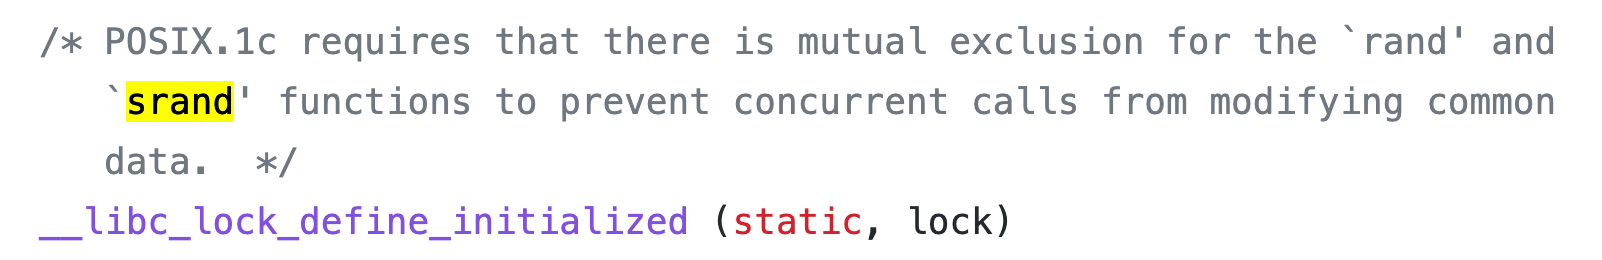
\includegraphics[width=0.4\textwidth]{random_function.png}
	\vspace{-1em}
	\caption{Random function bottleneck}
	\label{fig:random_function}
\end{figure}

As a result, we removed it when running the solver. This produced linear speedup up to 40 threads (on the psc machine), which is the number of first layer nodes. The graphs for search time and speedup with the increase of threads is shown in Fig \ref{fig:search_time_1} and Fig \ref{fig:speedup_1}, respectively. A problem with this approach is that it is difficult to parallelize with more threads using the current method because the number of first layer nodes is limited to 40. This is a major shortcoming since we should be able to perform 128-thread parallelization and much better speedup on the psc machines. To solve this issue, we decided on two alternative ways to perform parallelization: 1) rewrite the DFS parallel solver to map the workload onto the available threads (128 on the psc machines) and 2) perform the parallelization with Cilk instead of OpenMP. This brings us to our next approaches.

\subsection{Approach 2}

In this approach, instead of using DFS, we first calculate the number of possible leaf nodes, in the most naive case, it would be $40^{4}$ nodes. We then index this $40^{4}$ nodes and assign partition of the index to the worker threads where each worker thread is responsible for their assigned partition. For example, if there are 2560000 ($40^{4}$) nodes, each thread would be assigned 20000 nodes, so threads 0 would be responsible for node 0-19999, thread 1 responsible for node 20000-39999, and so on. Now the next problem is how do we map the node to the orientation and column position that should be dropped? We solve this by coming up with a one by one mapping function from the orientations and drop column position to the node id. We first consider there are four next blocks $T_{1}$, $T_{2}$, $T_{3}$ and $T_{4}$. Since we might prune redundant position, a tetris block might have less than 40 possible position. We let $O_{i}$ and $C_{i}$ be the number of possible orientation and drop column of tetromino block $T_{i}$, then the number of possible position of $T_{i}$ would be $O_{i} \cdot C_{i}$ which we annotate as $P_{i}$. Now the number of possible placement of all fours blocks would be $P_{1} \cdot P_{2} \cdot P_{3} \cdot P_{4}$. The next thing we do is we map the orientation $o_{i}$ and drop column $c_{i}$ of $T_{i}$ to a integer $tid_{i}$ where we define it as the tetris block id. We can achieve this easily by defining $$tid_{i} = o_{i} \cdot C_{i} + c_{i}$$ where both $o_{i}$, $c_{i}$ are integer and $o_{i} \in \interval[{0,O_{i}-1]$, $c_{i} \in \interval[{0,C_{i}-1]$.
Now consider the DFS case, every leaf node actually represent a combination of $tid_{i}$, hence we can map a leaf node to a set $\{ tid_{1}, tid_{2}, tid_{3},tid_{4}\}$. Finally, we can map this set to the node id we defined previously by the formula $$ id_{node} = tid_{1} \cdot  P_{2} \cdot P_{3} \cdot P_{4} + tid_{2} \cdot P_{3} \cdot P_{4} + tid_{3} \cdot P_{4} + tid_{4}$$
Using the formula, workers threads can easily map their given node id to the corresponding tetromino block placements using division and modulus. The synchronization overhead in this approach is neglectable since all threads first store the optimal solution of their partition to a local variable. The local optimal solution is then compared in a critical section to get the global optimal, which is very fast since it needs only the number of threads amount of comparison. This approach is much more flexible than approach one since we are now partitioning the node ids which is trivial to do, and allows us to do various optimization on the search space without changing our algorithm. It is also more efficient implementation-wise since we only need to recover the board state every 4 steps, unlike in the DFS case, where we need to do this for every new node. In the final version, we applied various optimization to push the perforamce to the limit, we would discuss them in the following section.
\subsection{Approach 3}

The other alternative for increasing the number of parallelization threads is to use Cilk. Cilk is the ideal parallelization tool given the recursive nature of our DFS solver. One advantage is the simplicity to convert C code to utilize Cilk, and the second advantage has to do with the workload imbalance due to pruning the redundant states mentioned in the background section.

First, we built CilkPlus on the GHC machine by building our own llvm with cmake via miniconda. The modifications we made to convert the code to Cilk includes using $cilk\_for$ to parallelize across different states of a level of search space (different positions and orientations). For each level, the DFS algorithm has to compare the scores obtained across different threads to find the optimal position and orientation. At first, we collected the scores from all threads using an array, and synchronized the threads with the $cilk\_sync$ barrier before performing a serialized comparison for all scores to find the best one. Then, we found that the cilk reducer \ref{ref:CilkReducer}, which is available only in C++, could be used to perform the same function without using synchronization and serialized comparison. Switching to the Cilk reducer speeds up the search time and reduces the amount of memory used since we do not need to keep track of scores form all threads.

Since there are redundant states as mentioned above, pruning them for optimization would cause workload imbalance. This would not be a problem with Cilk, since it has a work-stealing scheduler that would automatically balance the workload. A small problem we encountered is that we could not manually install CilkPlus on the PSC machines as we did on the GHC machines, because the gcc versions on the PSC machines are too recent. Therefore, we did not conduct our experiments of this approach on the PSC machines.

